\chapter{Methodology}
\label{ch:methods}

\section{Overview of the Proposed Method}

Considering the quality of journals in which an author's works are published
can notably assist in enhancing the accuracy and reliability of assessing their
scientific impact. Journal quality, often gauged by metrics such as the Journal
Impact Factor (JIF), which measures the importance of a journal and reputation
within the academic community by calculating the number of times selected
articles are cited within a particular year, plays a crucial role in how
citations are distributed and perceived \cite{garfield1999journal,
      garfield2006history}. For example, a JIF of 1.0 means that, on average,
articles published one or two years ago have been cited one time, while a JIF
of 2.5 means that articles have been cited 2.5 times on average. A higher
impact factor for a journal indicates that more of the journal's publications
have been highly cited, which suggests a higher quality of research being
published in the journal. This can be explained by the fact that high-impact
journals generate more citations due to their wide readership, rigorous
peer-review process, and the prestigious nature of the publications they
attract \cite{garfield2006history}.

Similarly, journals with higher h-index values tend to have a higher proportion
of highly cited papers, which indicates that the journal is publishing
high-quality research that is widely recognized and respected by the scientific
community. For example, a journal with a high h-index may have published
numerous papers that have been cited many times, indicating that the research
is influential and widely accepted. On the other hand, a journal with a
low h-index may have published fewer highly cited papers, suggesting that the
research is less influential or less well-received by the scientific community.

More recently, the EigenFactor metric has emerged as an alternative measure of
journal quality, which evaluates the influence of a journal based on the number
of incoming citations, with citations from highly influential journals being
weighted more heavily than those from less influential ones. It was designed to
address the limitations of traditional citation metrics like the Impact Factor
(JIF), which can be skewed by a few highly cited papers, by leveraging the
structure of citation networks \cite{bergstrom2007eigenfactor}.

In detail, the EigenFactor is calculated by analyzing the network of academic
citations among journals. It employs an algorithm similar to Google's PageRank
\cite{rogers2002google} to measure the importance of journals based on their
citations, and the process involves creating a matrix that records how often
each journal cites every other journal. Using this matrix, the algorithm
simulates a random walk through the citation network, where a hypothetical
researcher selects articles and follows their citations to other journals
repeatedly. This random walk model helps determine the frequency with which a
researcher would visit each journal, reflecting its overall influence. Finally,
the EigenFactor Score is derived from these visitation frequencies, giving more
weight to citations from prestigious journals, and adjusting for differences in
citation practices across various fields \cite{Bergstrom11433, Alan2009}.

Having the above in mind, when evaluating an author's h-index, it could be
beneficial to focus on their publications in reputable journals with high
impact factors, eigenfactors or h-index values, which helps to exclude
publications of questionable quality, thus better reflecting the significance
and recognition of the author's contributions to their field.

The proposed method aims to address the problem of h-index inflation by
developing three novel metrics that adjust for the subject area and the quality
of the journal in which the work is published. The first metric, the
\textit{Adjusted h-index} ($h_{\text{adj}}$), adjusts the h-index by only
considering publications from the top 20\% of journals in its corresponding
subject area, based on the H5 index of the journal. The second metric, the
\textit{JIF-adjusted h-index} ($h_{\text{JIF}}$), adjusts the h-index
similarly, but the ranking of the journals is determined by the Journal Impact
Factor (JIF) in which the publication is published. Lastly, the
\textit{Eigenfactor-adjusted h-index} ($h_{\text{EF}}$), adjusts the h-index by
considering the EigenFactor of the journal. The proposed methods are
implemented in \emph{SQL} and the data is stored in a \emph{Sqlite} database,
with only the EigenFactor calculation being done in \emph{Python}.

\section{Data Collection and Preprocessing}

For the purpose of this study, the Alexandria3k \cite{Spi23g} package was used
to collect publication data from the Crossref dataset \cite{Crossref2020} and
prepare it for processing. The Crossref dataset is known for its comprehensive
and standardized approach to indexing publications across a wide range of
disciplines, which is helpful for reducing discrepancies that might arise from
varying data formats used by different databases (Scopus, Web of Science,
etc.). Crossref collaborates with a large number of publishers to ensure that a
wide range of academic content is covered, including journal articles,
conference proceedings, and other scholarly works.

Alexandria3k supplies a library and a command-line tool providing efficient
relational query access to diverse publication open data sets. Specifically,
the dataset that was used is a subset of the Crossref-2024 dataset along with
the subjects of journals (from the 2024 subset) from the Crossref-2023 dataset,
where the whole Crossref-2024 contains publication metadata from about 156
million publications from all major international publishers with full citation
data for around 60 million of them. Using our subsets, we are checking around
1.5 million publications, which are the publications in the period 2019--2023.
In addition to that, for the subject of the publications, the Scopus ASJC (All
Science Journal Classification) subject codes were used.

To be more specific, the ASJC codes were used to categorize the publications
into more general subject areas than the original areas provided by the
Crossref-2023 dataset. The ASJC codes are a standard classification system used
to categorize publications into subject areas and are widely used in the
scientific community. These codes are hierarchical and are organized into four
levels, with the first level being the broadest and the fourth level being the
most specific. For the purpose of this study, the first level of the ASJC codes
was used to categorize the publications into broad subject areas, so the
analysis could be generalized across different disciplines, without getting
lost in the details of subfields. Crucial to note is that the codes are not
available for publications in the Crossref-2024 dataset
\cite{crossrefSubjectCodes2024}, so only journals with subjects from the 2023
dataset or with subjects retrievable using the Scopus API
\cite{elsevier_dev_portal} were considered for this study, since for those
journals the codes were retrievable.

\section{Implementation of the Proposed Methods}

The proposed method was implemented in SQL using the \emph{SQLite} database
management system. The implementation consists of three main parts: the
calculation of the Adjusted h-index and the EigenFactor-adjusted h-index based
on the last 5 years, along with the calculation of the JIF-adjusted h-index
based on the last 3 years. All methods share the same structure and similar
preparation steps, with the main difference being the metrics (H5, IF3 and
EigenFactor) used to rank the journals. In order to use the subject codes from
the Scopus ASJC classification, since they are not available in the
Crossref-2024 dataset, the journals (ISSN) along with their subject codes were
extracted from the 2023 version and stored in a separate table (called
journal\_data). Additionally, if the ASJC codes were not available for a
journal, even from the 2023 dataset, the Scopus API was used to retrieve the
subject codes, if possible. After that, the preparation of the database
involved creating tables to store and index works and authors.

Important to note is that, for the consideration of the 'lower quality'
journals for the Adjusted h-index and the JIF-adjusted h-index, the bottom 50\%
of journals were considered, while the bottom 20\% of journals were considered
for the EigenFactor adjusted h-index, due to the different distribution of the
EigenFactor scores compared to rest of the indexes. Specifically, the
EigenFactor allows a broader range of journals to be considered lower-tier,
being potentially more sensitive to journal quality and, thus, able to capture
differences in it more effectively than the previous indexes. This led to the
decision to consider only the bottom 20\% for the EigenFactor adjusted h-index,
in order to be comparable with our criteria for the H5 and JIF adjusted
h-indexes for what was considered to be journals of lesser quality.

\subsection{Calculation of the Adjusted h-index}

\begin{enumerate}
      \item \textbf{Count Citations for Each Work}: Calculate the number of citations for each work to determine its impact.

      \item \textbf{Calculate the h5 Index of Journals}: Derive the h5 index for journals, which is a
            measure of their citation impact over the past five years.

      \item \textbf{Identify the Top 20\% of Journals by Subject Based on the h5 Index}: Determine the top 20\% of journals within
            each subject area based on their h5 index.

      \item \textbf{Filter Works from the Top Journals by Subject}: Generate tables that include works from the
            top journals for each subject area, ensuring that only high-impact works are considered.

      \item \textbf{Calculate the Adjusted h-index for Each Author}: Determine the adjusted h-index for each author,
            taking into account the subject area of each authors works.
\end{enumerate}

\subsection{Calculation of the JIF-adjusted h-index}
\begin{enumerate}
      \item \textbf{Calculate Work Citations}: Compute the number of citations for each work to assess their impact.

      \item \textbf{Filter Citable Works}: Identify works that are longer than two pages to exclude non-research articles such as news or book reviews.

      \item \textbf{Calculate the Number of Publications in the Impact Factor (IF) Period}: Count the number of publications
            for each journal within the IF period (last 3 years).

      \item \textbf{Calculate the Journal Impact Factor (JIF)}: Derive the JIF by dividing the number of citations by
            the number of publications for each journal.

      \item \textbf{Identify the Top 20\% of Journals by Subject Based on JIF}: Select the top 20\% of journals within
            each subject area based on their JIF\@.

      \item \textbf{Filter Works from the Top Journals by Subject}: Generate tables that include works from
            the top journals for each subject area, ensuring that only high-impact works are considered.

      \item \textbf{Calculate the Adjusted h-index for Each Author}: Determine the adjusted h-index for each author.
\end{enumerate}

\subsection{Calculation of the EigenFactor-adjusted h-index}
\begin{enumerate}
      \item \textbf{Derive the Citation Network of Journals}: Create a citation network of journals based on the
            incoming citations to each journal from the past 5 years.
      \item \textbf{Calculate the EigenFactor of Journals}: Calculate the EigenFactor of each journal based on the
            citation network, based on the steps
            described from the official EigenFactor pseudo-code \cite{west2008pseudocode}. The calculations were done  in Python
            3.11.9, using the \emph{NumPy} library for the matrix operations and the
            calculation of the leading eigenvector, along with the \emph{Pandas} library
            for data manipulation.
      \item \textbf{Identify the Top 20\% of Journals by Subject Based on EigenFactor}: Select the top 20\% of journals within
            each subject area based on their EigenFactor score\@.

      \item \textbf{Create Filtered Works Tables from the Top Journals by Subject}: Generate tables that include works from
            the top journals for each subject area, ensuring that only high-impact works are considered.

      \item \textbf{Calculate the Adjusted h-index for Each Author}: Determine the adjusted h-index for each author.
\end{enumerate}

\section{ROLAP Analysis}

The proposed method was implemented using a Relational Online Analytical
Processing (ROLAP) approach. ROLAP is a database management system that enables
users to analyze multidimensional data stored in a relational database
\cite{codd1993providing}. The implementation of the proposed method in ROLAP
allows for efficient querying and analysis of the publication data to calculate
the adjusted h-indexes. For the ROLAP implementation, the tool
\emph{simple-rolap} \cite{simple-rolap} was used, which provides a simple
framework for maintainable and time-efficient ROLAP by enabling the
specification of small, modular SQL queries. It is designed for querying rarely
modified data sets and is particularly useful in scenarios where materialized
views are unsupported or unusable.

The primary function of \emph{simple-rolap} is to save the result of each SQL
query in corresponding tables, which can then be used by subsequent queries.
This modular approach allows for the independent development and testing of
each query. Additionally, its automatic dependency analysis feature, ensures
that new queries can utilize already calculated results and that when a query
is changed, only the dependent tables are automatically repopulated.

\section{Testing of the Proposed Method}
For the testing of the proposed methods, the \emph{RDBUnit} \cite{rdbunit}
library was used to create and execute unit tests. \emph{RDBUnit} is a database
unit testing framework that allows for the creation of test cases for SQL
queries and stored procedures. It provides a simple and efficient way
to express the setup prior to a query, the query itself, and the expected
results. This framework can test \texttt{SELECT} queries as well as queries
used for creating tables and views, offering flexibility in how tests are
structured.

\emph{RDBUnit} enables the embedding of all types of queries directly into the test
script or the inclusion of queries from external files. It streamlines the
creation of input and expected result tables by automatically inferring the
types of the tables' fields, thus reducing the overhead typically associated
with setting up test environments. This makes it an ideal choice for
ensuring the accuracy and reliability of SQL queries used in the proposed
methods, enhancing the overall robustness of the calculations.

\section{Detailed Calculation of the Adjusted h-indexes}

In detail, for the calculation of the Adjusted h-indexes, the SQL tables are as
follows:

\subsection{Data from Crossref-2024 Dataset}
\begin{itemize}
      \item \textbf{Works}: Contains the works with their respective DOIs and the number of citations.
      \item \textbf{Authors}: Contains the authors with their respective ORCID identifiers.
      \item \textbf{Journals (journal\_data)}: Contains the journals with their respective ISSNs and subject areas.
      \item \textbf{ASJC}: Contains the ASJC codes for the subject areas that were extracted from the Crossref-2023 dataset.
      \item \textbf{Work References}: Contains the references of the works.
\end{itemize}

\subsection{ROLAP Analysis Tables}

\noindent\textbf{1: Data Preparation}
\begin{itemize}
      \item \textbf{works\_orcid}: Contains the works with their respective authors.
      \item \textbf{works\_issn\_subject}: Contains the journals with their respective subject areas, in AJSC codes.
      \item \textbf{work\_citations}: Contains the works with their respective citations.
\end{itemize}

\vspace{0.5em} % Add space to separate the comment
\noindent\emph{For Impact Factor calculation only:}
\begin{itemize}
      \item \textbf{Citations}: Contains the works that were published in the last year and cited from works published in the last two years.
      \item \textbf{Citable\_Works}: Contains the works that are longer than two pages.
      \item \textbf{Publications}: Contains the number of publications for each journal within the IF period.
\end{itemize}

\vspace{0.5em} % Add space to separate the comment
\noindent\emph{For EigenFactor calculation only:}
\begin{itemize}
      \item \textbf{Citation\_Network}: Contains the citation network of journals based on the incoming citations to each journal of the past 5 years.
\end{itemize}

\noindent\textbf{2i: Calculation of Journal h5 Index}
\begin{itemize}
      \item \textbf{issn\_subject\_h5}: Calculates the h5 index of the journals.
\end{itemize}

\noindent\textbf{2ii: Calculation of Journal Impact Factor (JIF)}
\begin{itemize}
      \item \textbf{impact\_factor}: Calculates the Journal Impact Factor (JIF).
\end{itemize}

\noindent\textbf{2iii: Calculation of Journal EigenFactor}
\begin{itemize}
      \item \textbf{eigenfactor\_scores}: Contains the EigenFactor for each journal, calculated using Python and then inserted into the ROLAP database.
\end{itemize}

\noindent\textbf{3: Getting Top and Bottom Percentile of Journals}
\begin{itemize}
      \item \textbf{top\_issn\_by\_subject}: Contains the top 20\% of journals by subject based on the h5 index or the JIF.
      \item \textbf{bottom\_issn\_by\_subject}: Contains the bottom 50\% of journals by subject based on the h5 index or the JIF, or 
            the bottom 20\% of journals by subject based on the EigenFactor.
\end{itemize}

\noindent\textbf{4: Filtered Works Tables}
\begin{itemize}
      \item \textbf{filtered\_works\_orcid}: Contains the works from the top journals by subject.
      \item \textbf{bottom\_filtered\_works\_orcid}: Contains the works from the bottom journals by subject.
\end{itemize}

\noindent\textbf{5: Calculation of the Adjusted h-index}
\begin{itemize}
      \item \textbf{orcid\_h5\_filtered}: Calculates the h5 index for each author regarding their discipline (subject area).
      \item \textbf{orcid\_h5\_bottom}: Calculates the h5 index for each author from the 'lower quality' journals.
\end{itemize}

Figure \ref{fig:tables} shows the dependencies of each table for the
implementation of the Adjusted h-index by filtering the top 20\% of journals by
subject based on the h5 index.

\begin{figure}[H]
      \centering
      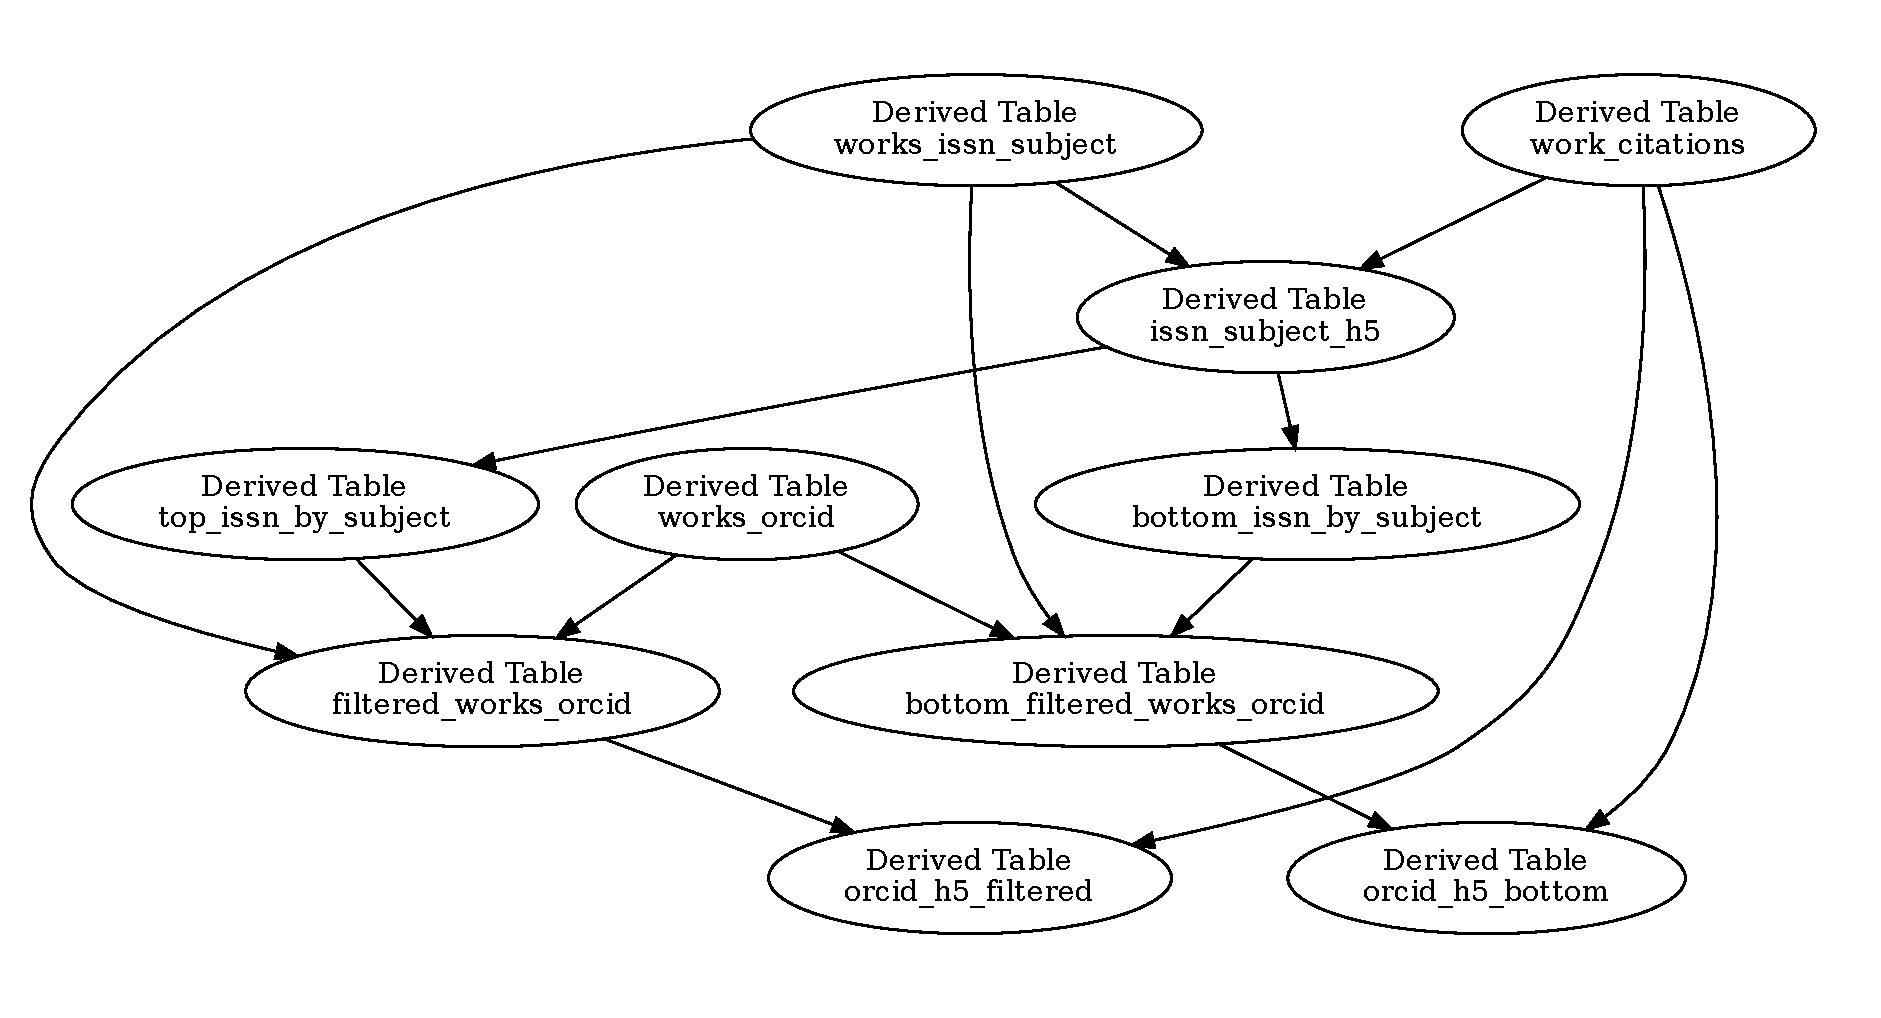
\includegraphics[width=0.8\textwidth]{../figs/h5.pdf}
      \caption{Dependencies of the tables used in the implementation of the Adjusted h-index by filtering the top 20\% and bottom 50\% of journals by subject based on the h5 index.}
      \label{fig:tables}
\end{figure}

Figure \ref{fig:tables2} shows the dependencies of each table for the
implementation of the JIF-adjusted h-index by filtering the top 20\% of
journals by subject based on the Journal Impact Factor (JIF).

\begin{figure}[H]
      \centering
      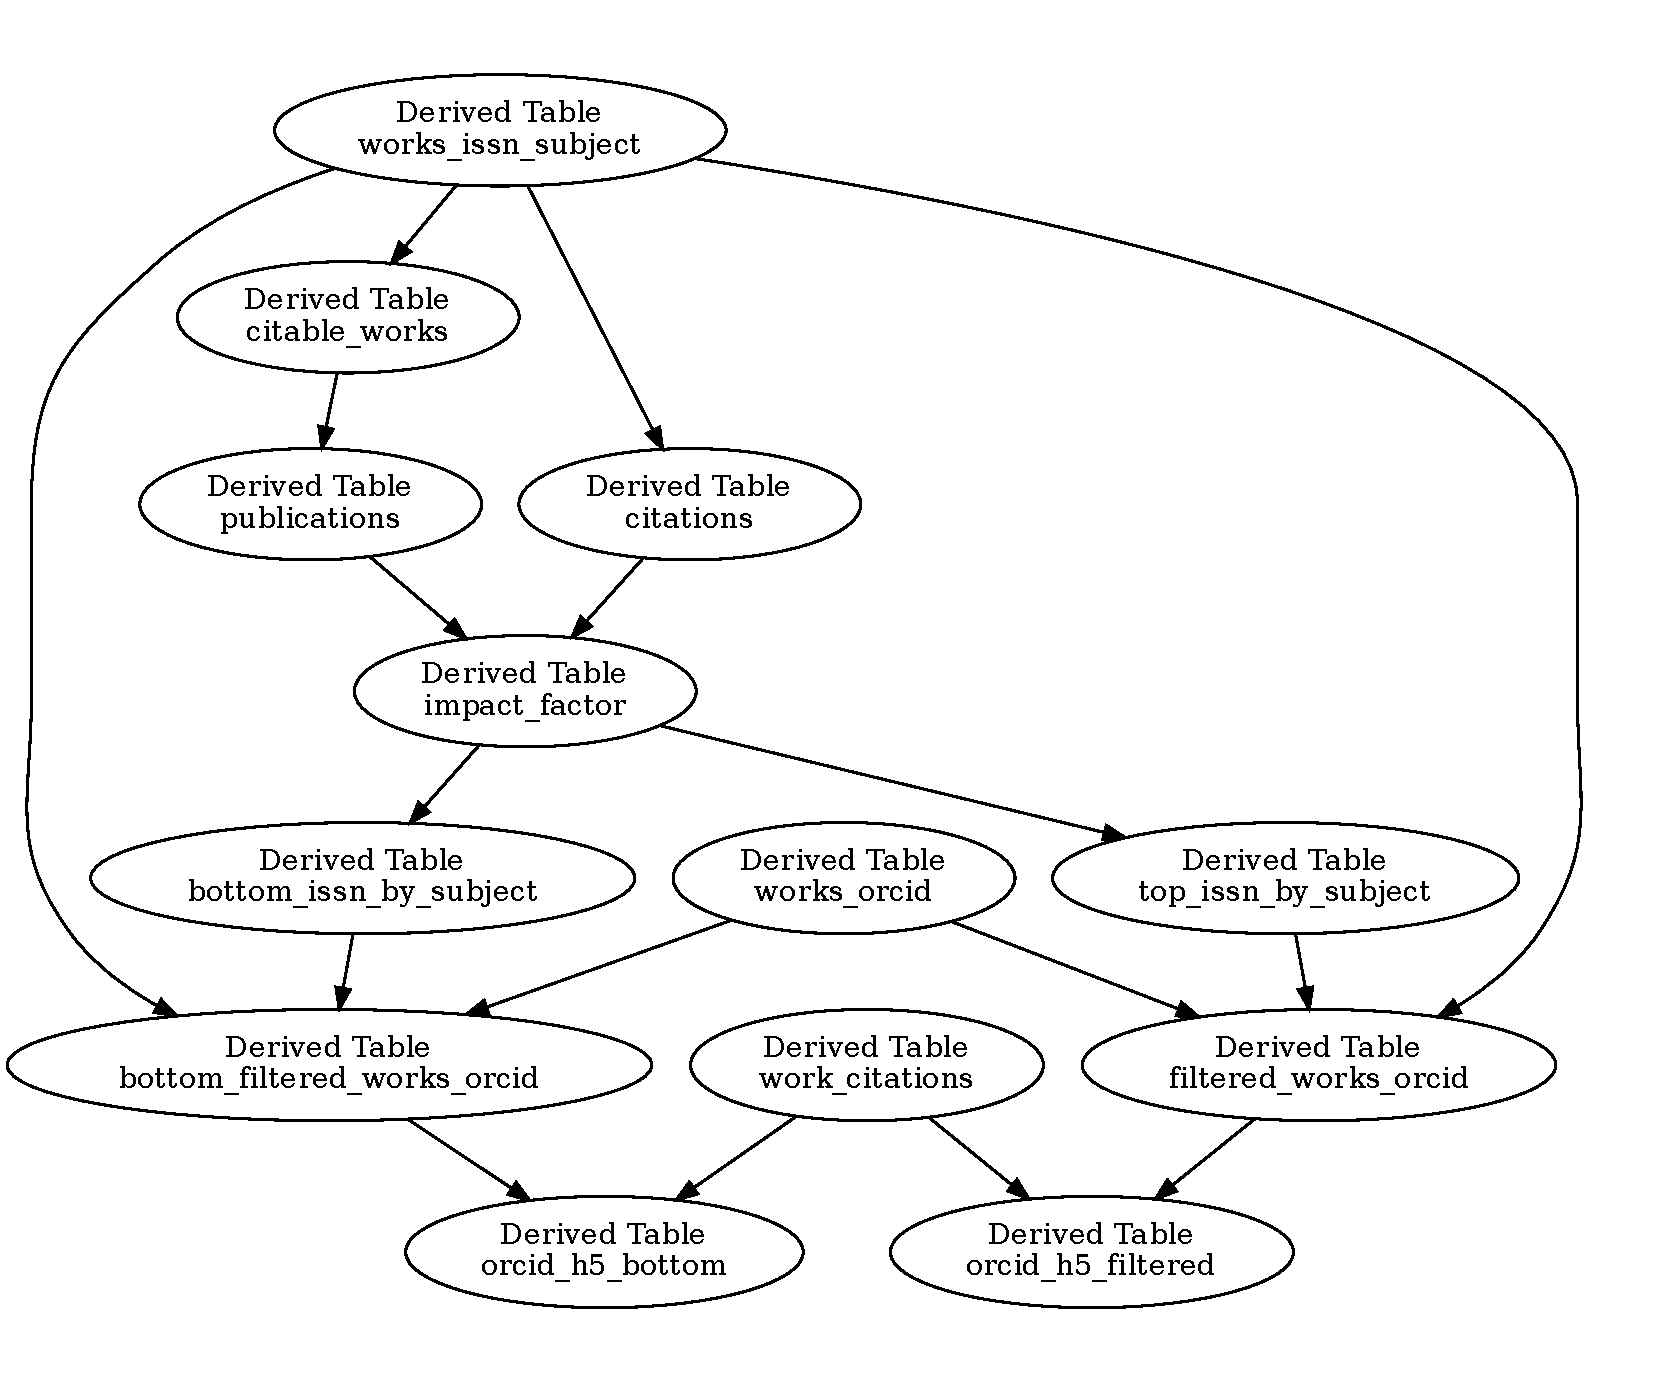
\includegraphics[width=0.8\textwidth]{../figs/impact.pdf}
      \caption{Dependencies of the tables used in the implementation of the JIF-adjusted h-index by filtering the top 20\% and bottom 50\% of journals by subject based on the Journal Impact Factor (JIF).}
      \label{fig:tables2}
\end{figure}

Figure \ref{fig:tables3} shows the dependencies of each table for the
implementation of the EigenFactor-adjusted h-index by filtering the top 20\% of
journals by subject based on the EigenFactor.

\begin{figure}[H]
      \centering
      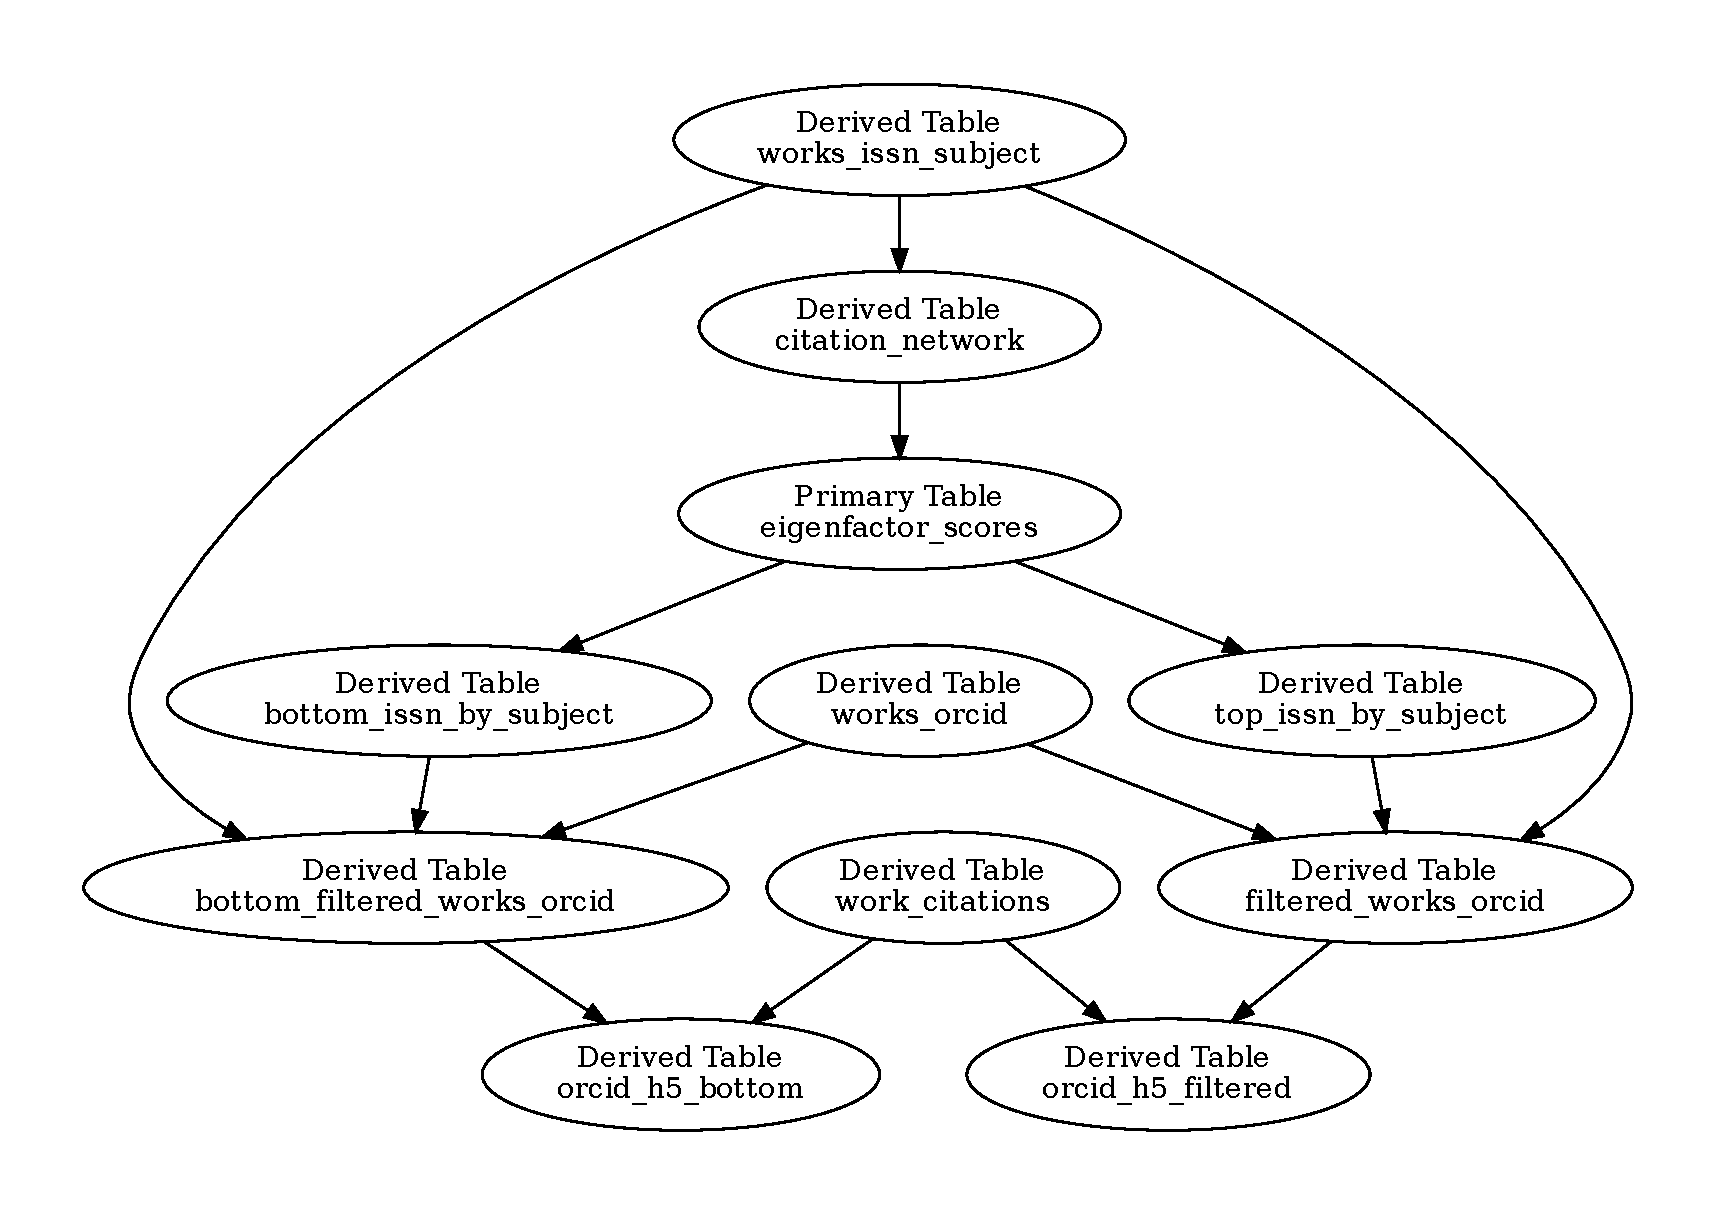
\includegraphics[width=0.8\textwidth]{../figs/eigenfactor.pdf}
      \caption{Dependencies of the tables used in the implementation of the EigenFactor-adjusted h-index by filtering the top 20\% and bottom 20\% of journals by subject based on the EigenFactor.}
      \label{fig:tables3}
\end{figure}

